\documentclass[tikz,border=2pt]{standalone}
\usepackage{amsmath}
\usepackage{pgfplots}
\pgfplotsset{compat=1.18}
\usetikzlibrary{arrows.meta}
\begin{document}
% Example 6.2/7.2: max c_1x_1+5x_2 s.t. x_1<=4, 2x_2<=12, 3x_1+2x_2<=18. The objective line through (2,6)
% has slope -c_1/5; (2,6) stays optimal while it lies between the edge slopes 0 (c_1=0) and -3/2 (c_1=15/2).
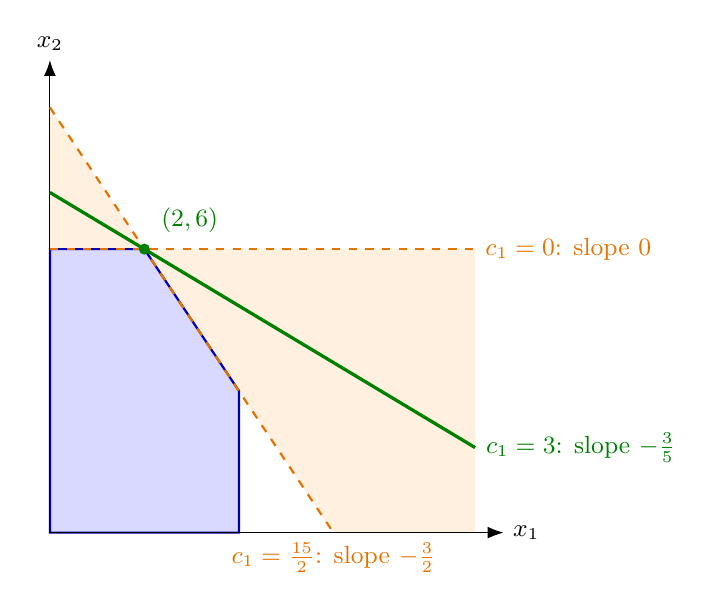
\begin{tikzpicture}[font=\small, >={Latex[length=2mm]}, x=0.6cm, y=0.6cm]
  % double wedge of objective lines through (2,6) that keep the corner optimal
  \fill[orange!12] (2,6) -- (9,6) -- (9,0) -- (6,0) -- cycle;
  \fill[orange!12] (2,6) -- (0,6) -- (0,9) -- cycle;
  % feasible region
  \fill[blue!15] (0,0) -- (4,0) -- (4,3) -- (2,6) -- (0,6) -- cycle;
  \draw[blue!70!black, thick] (0,0) -- (4,0) -- (4,3) -- (2,6) -- (0,6) -- cycle;
  % axes
  \draw[->] (0,0) -- (9.6,0) node[right] {$x_1$};
  \draw[->] (0,0) -- (0,10) node[above] {$x_2$};
  % limiting objective lines (they contain the two edges at (2,6))
  \draw[orange!90!black, thick, dashed] (0,6) -- (9,6) node[right] {$c_1=0$: slope $0$};
  \draw[orange!90!black, thick, dashed] (0,9) -- (6,0) node[below] {$c_1=\tfrac{15}{2}$: slope $-\tfrac{3}{2}$};
  % current objective line 3x_1+5x_2=36
  \draw[green!50!black, very thick] (0,7.2) -- (9,1.8) node[right] {$c_1=3$: slope $-\tfrac{3}{5}$};
  % optimal corner
  \fill[green!50!black] (2,6) circle (2pt);
  \node[green!50!black, anchor=south west] at (2.15,6.15) {$(2,6)$};
\end{tikzpicture}
\end{document}
